\documentclass[]{article}
\usepackage{amsmath}
\usepackage{graphicx} 

%opening
\title{GPU Gradient Decent Shape Optimizer Design}
\author{}

\begin{document}
	
\maketitle
	
	
\section{Requirements}
Write a GPU accelerated shape optimizer to practice GPU optimizations and investigate speed up for Morpho first version should be able to:
\begin{itemize}
	\item Optimize surface Area with constant Volume
	\item Read in morpho meshes (for ease of use)
	\item Run on the GPU
	\item Input is Morpho mesh print area and volume. output is optimized morpho mesh print area and volume
\end{itemize}
	
\section{Conceptual Method}
A mesh is a list of vertices $\vec{r_i}$ with rules for how the connect. One dimensional connections are lines, Two dimensional connections are facets. A connection is a list of vertex indices that are part of the higher dimensional element. Let $i$ label verties, $k$ label facets and $l$ label the vertex in a facet.
Consider a facet $f_k$ with three vertices labeled $\vec{r}_{f_{k_l}}$ I.E $\vec{r}_{f_{k_1}},\vec{r}_{f_{k_2}}\vec{r}_{f_{k_3}}$. The area of this facet is:
$$A_k = (\vec{r}_{f_{k_2}} - \vec{r}_{f_{k_1}}) \times  (\vec{r}_{f_{k_3}} - \vec{r}_{f_{k_2}})$$
To minimize area we need to find the gradient of the area with respect to the vertices of the facet.
\begin{align}
	\vec{S}_0 &=  (\vec{r}_{f_{k_2}} - \vec{r}_{f_{k_1}})\\
	\vec{S}_1 &= (\vec{r}_{f_{k_3}} - \vec{r}_{f_{k_2}})\\
	\vec{S}_{01} &= \vec{S}_0\times \vec{S_1}\\
	\vec{S}_{010} &= \vec{S}_{01}\times \vec{S}_0\\
	\vec{S}_{011} &= \vec{S}_{01}\times \vec{S}_1\\
	\nabla_{\vec{r}_{f_{k_1}}}A_{f_k} &=  \frac{\vec{S}_{011}}{2 |\vec{S}_{01}|}\\
	\nabla_{\vec{r}_{f_{k_2}}}A_{f_k} &=  -\frac{\vec{S}_{011}+\vec{S}_{010}}{2 |\vec{S}_{01}|}\\
	\nabla_{\vec{r}_{f_{k_3}}}A_{f_k} &=  \frac{\vec{S}_{010}}{2 |\vec{S}_{01}|}
\end{align}
Now that we have the area per vertex per facet we need to collate them to find the gradient. To do this on the GPU avoiding write collisions we use a map from $F(i):i\rightarrow{(k,l)_{m_i}}$ where $m_i$ counts up to the number of facets vertex $i$ is included in. The gradient of the are with respect to a single vertex $i$ is then:
$$\nabla_{\vec{r}_i} A = \sum_{(k,l)_{m_i}} \nabla_{\vec{r}_{f_{k_l}}}A_{f_k}$$

Likewise for volume integrand on a facet we have
$$V_{f_{k}} = \left|\frac{(\vec{r}_{f_{k_1}} \times \vec{r}_{f_{k_2}}) \cdot \vec{r}_{f_{k_3}}}{6}\right|$$

The gradient of the volume integrad for each vertex on a facet is then
\begin{align}
s &= sign((\vec{r}_{f_{k_1}} \times \vec{r}_{f_{k_2}}) \cdot \vec{r}_{f_{k_3}})\\
\nabla_{\vec{r}_{f_{k_1}}}V_{f_k} &=\frac{s}{6}\vec{r}_{f_{k_2}} \times \vec{r}_{f_{k_3}}\\
\nabla_{\vec{r}_{f_{k_2}}}V_{f_k} &=\frac{s}{6}\vec{r}_{f_{k_3}} \times \vec{r}_{f_{k_1}}\\
\nabla_{\vec{r}_{f_{k_3}}}V_{f_k} &=\frac{s}{6}\vec{r}_{f_{k_1}} \times \vec{r}_{f_{k_2}}
\end{align}
Then we perform the sum in the same manor 
$$\nabla_{\vec{r}_i} V = \sum_{(k,l)_{m_i}} \nabla_{\vec{r}_{f_{k_l}}}V_{f_k}$$

To minimize area with constant volume we project the area gradient vector to the space where the volume change is zero. We call the negative of this projection the force. 
$$ \vec{F}_i = -\left(\nabla_{\vec{r}_i} A - \frac{\nabla_{\vec{r}_i} A \cdot \nabla_{\vec{r}_i} V}{\nabla_{\vec{r}_i} V \cdot \nabla_{\vec{r}_i} V}\nabla_{\vec{r}_i} V\right)$$

Gradient decent then consists of calculating this force and moving the vertices on the mesh until the force is below a threshold value. 

\section{Implementation Method}
First pass of this will be done in C++ using CUDA for GPU acceleration Class stucture is below
\begin{figure}[h]
	\centering
	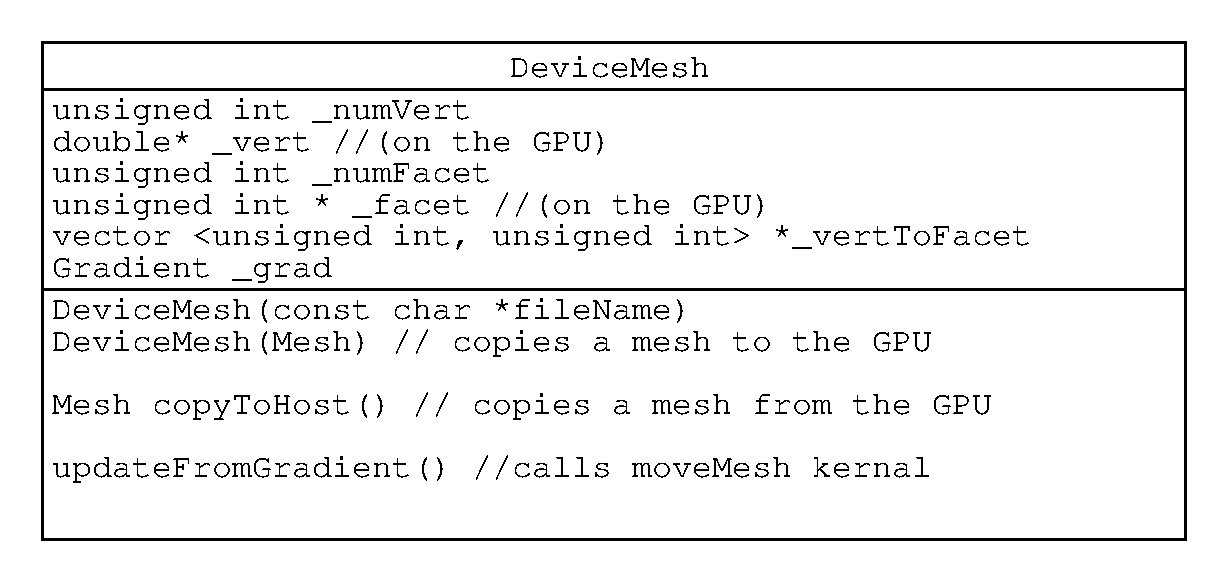
\includegraphics[width=1\linewidth]{Classes}
	\caption[Class Diagram]{For this project there will be a optimizer class that manages a gradient and a mesh to perform the optimization. It will load in a mesh from file, create a device mesh from this mesh and tell the gradients to calculate and the mesh to move.}
	\label{fig:classes}
\end{figure}

\end{document}

